\chapter{Direct and Statistical Testing Methods for Selecting $K$}\label{mywork}

\section{Introduction}
Determining the number of clusters in a data set, a quantity often labelled $K$ as in the $K$-means algorithm,
is a frequent problem in data clustering, and is a distinct issue from the process of actually solving the
clustering problem. Clustering solutions may vary as different numbers of clusters are specified.
A clustering technique would most possibly recover the underlying cluster structure given a good
estimate of the true number of clusters.

For a certain class of clustering algorithms (in particular k-means, k-medoids and expectation–maximization algorithm),
there is a parameter commonly referred to as $K$ that specifies the number of clusters to detect. Other algorithms such
as DBSCAN and OPTICS algorithm do not require the specification of this parameter; hierarchical clustering avoids the
problem altogether.

The correct choice of $K$ is often ambiguous, with interpretations depending on the shape and scale of the distribution
of points in a data set and the desired clustering resolution of the user. In addition, increasing $K$ without penalty
will always reduce the amount of error in the resulting clustering, to the extreme case of zero error if each data point
is considered its own cluster (i.e., when $K$ equals the number of data points, n). Intuitively then, the optimal choice
of $K$ will strike a balance between maximum compression of the data using a single cluster, and maximum accuracy by
assigning each data point to its own cluster. If an appropriate value of $K$ is not apparent from prior knowledge of the
properties of the data set, it must be chosen somehow. There are several categories of methods for making this decision.

A number of strategies for estimating the optimal number of clusters have been proposed.
A very extensive comparative evaluation was conducted by Milligan and Cooper~\cite{milligan85},
where they compared 30 proposed methods in estimating the true number of clusters
when applying hierarchical clustering algorithms to simulated data with well-separated clusters.
According to their work, Calinski and Harabasz’s index~\cite{Calinski1974} is the most effective one,
followed by Duda and Hart’s method~\cite{Hart73} and the C-index.

\section{Elbow Method}
The oldest method for determining the true number of clusters in a data set is inelegantly called the elbow method\index{Elbow Method}.
It's pure simplicity, and for that reason alone has probably been reinvented many times over (ed. note:
This is a problem peculiar to clustering; since there are many intuitively plausible ways to cluster data,
it's easy to reinvent techniques, and in fact one might argue that there are very few techniques in clustering
that are complex enough to be 'owned' by any inventor). The idea is this:

    Start with $k=1$, and keep increasing it, measuring the cost of the optimal quality solution.
    If at some point the cost of the solution drops dramatically, that's the true $k$.

The intuitive argument behind the elbow method is this: you're trying to shoehorn k boxes of data into many
fewer groups, so by the pigeonhole principle, at least one group will contain data from two different boxes,
and the cost of this group will skyrocket. When you finally find the right number of groups, every box fits
perfectly, and the cost drops.

Recall that, the basic idea behind partitioning methods, such as k-means clustering,
is to define clusters such that the total intra-cluster variation (known as total within-cluster
variation or total within-cluster sum of square) is minimized:\\\\
$minimize(\sum_{k=1}^{K}WC_k)$;

where $C_k$ is the $k^{th}$ cluster and $W(C_k)$ is the within-cluster variation.
That means the total within-cluster sum of square $(wss)$ measures the compactness of the clustering and we want
it to be as small as possible.

The optimal number of clusters can be defined as follow:

\begin{algorithm}
  \caption{Elbow Method}
  \label{alg1}
  \begin{algorithmic}
    \input{algorithms/elbow.alg}
  \end{algorithmic}
\end{algorithm}

\begin{figure}[t]
  \centering
  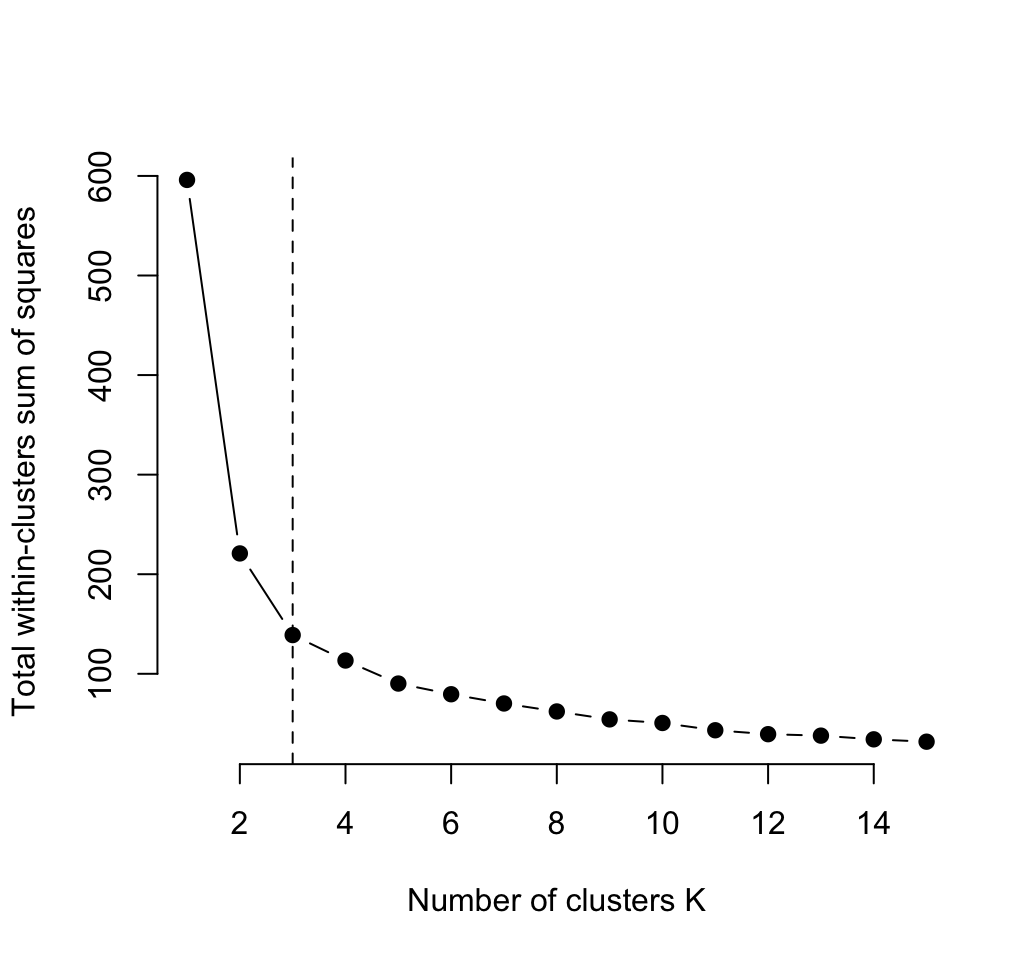
\includegraphics[width=0.9\textwidth]{figures/elbow1}
  \caption{Elbow Method Example}
  \label{fig:elbow}
\end{figure}

In Figure \ref{fig:elbow} we can see that Total within-clusters sum of squares have been plotted along
the Y-axis and Number of clusters $K$ along the X-axis. The bend(knee) in the graph is detected where
the value of $K$ is three. So, here in the example graph the elbow method suggests 3 cluster solutions.

It looks deceptively simple. But it has that aspect that we've mentioned earlier - it defines the desired outcome
as a transition, rather than a state. In practice of course, ``optimal quality" becomes ``whichever clustering
algorithm you like to run", and ``drops dramatically" becomes one of those gigantic hacks that make Principle and
Rigor run away crying and hide under their bed. So, here the problem  with  elbow  method is:  This  "elbow"  cannot
always  be  unambiguously  identified.  Sometimes  there  is  no  elbow,  or  several elbows

\section{Average Silhouette Method}
Silhouette\index{Average Silhouette Method} refers to a method of interpretation and validation of consistency within clusters of data.
The technique provides a succinct graphical representation of how well each object lies within its cluster.
It was first described by Peter J. Rousseeuw in 1987. Kaufman and Rousseeuw~\cite{rousseeuw90} proposed the
silhouette index as to estimate the optimum number of clusters in the data. The definition of the
silhouette index is based on the silhouettes introduced by Rousseeuw~\cite{rousseeuw87}, which are constructed
to show graphically how well each object is classified in a given clustering output.

The silhouette\index{Silhouette} value is a measure of how similar an object is to its own cluster (cohesion) compared to other
clusters (separation). The silhouette ranges from -1 to 1, where a high value indicates that the object is well
matched to its own cluster and poorly matched to neighboring clusters. If most objects have a high value, then
the clustering configuration is appropriate. If many points have a low or negative value, then the clustering
configuration may have too many or too few clusters.

The silhouette can be calculated with any distance metric, such as the Euclidean distance or the Manhattan distance.

\begin{itemize}
\item \textbf{Euclidean Distance} : The Euclidean distance\index{Euclidean Distance} between points p and q is the length of the line segment
connecting them $(\overline{\mathbf{p}\mathbf{q}})$. In Cartesian coordinates, if $p$ = ($p_1$, $p_2$,..., $p_n$) and $q$ = ($q_1$, $q_2$,..., $q_n$) are two points in Euclidean $n$-space,
then the distance $d$ from $p$ to $q$, or from $q$ to $p$ is given by the Pythagorean formula:

$d(p, q)$ = $\sqrt{\sum_{i=1}^{n}(q_i-p_i)^2}$

\item \textbf{Manhattan Distance} : The distance\index{Manhattan Distance} between two points measured along axes at right angles.
In a plane with $p_1$ at ($x_1$, $y_1$) and $p_2$ at ($x_2$, $y_2$), it is $|x_1 - x_2| + |y_1 - y_2|$.
\end{itemize}

Assume the data have been clustered via any technique, such as $K$-means, into $K$ clusters.
For each datum $i$, let $(i)$ be the average dissimilarity of $i$ with all other data within
the same cluster. We can interpret $a(i)$ as how well $i$ is assigned to its cluster (the
smaller the value, the better the assignment). We then define the average dissimilarity of
point $i$ to a cluster $c$ as the average of the distance from $i$ to all points in $c$.

Let $b(i)$ be the lowest average dissimilarity of $i$ to any other cluster, of which $i$ is
not a member. The cluster with this lowest average dissimilarity is said to be the ``neighbouring
cluster" of $i$ because it is the next best fit cluster for point $i$. We now define a silhouette:

$s(i) = \frac{b(i) - a(i)}{max(a(i), b(i))}$; where $-1\leq{s(i)}\leq{1}$

For $s(i)$ to be close to 1, we require $a(i)$ $\ll$ $b(i)$. As $a(i)$ is a measure of how dissimilar $i$
is to its own cluster, a small value means it is well matched. Furthermore, a large $b(i)$ implies that $i$
is badly matched to its neighbouring cluster. Thus an $s(i)$ close to one means that the data is appropriately
clustered. If $s(i)$ is close to negative one, then by the same logic we see that $i$ would be more appropriate
if it was clustered in its neighbouring cluster. An $s(i)$ near zero means that the datum is on the border of
two natural clusters.

The average $s(i)$ over all data of a cluster is a measure of how tightly grouped all the data in the cluster are.
Thus the average $s(i)$ over all data of the entire dataset is a measure of how appropriately the data have been
clustered. If there are too many or too few clusters, as may occur when a poor choice of $K$ is used in the
clustering algorithm (e.g.: $K$-means), some of the clusters will typically display much narrower silhouettes
than the rest. Thus silhouette plots and averages may be used to determine the natural number of clusters
within a dataset. One can also increase the likelihood of the silhouette being maximized at the correct number
of clusters by re-scaling the data using feature weights that are cluster specific ~\cite{hennig15}.

The average silhouette approach we'll be described comprehensively in the chapter cluster validation statistics.
Briefly, it measures the quality of a clustering. That is, it determines how well each object lies within its
cluster. A high average silhouette width indicates a good clustering. The algorithm is similar to the elbow
method and can be computed as follow:

\begin{algorithm}
  \caption{Silhouette Method}
  \label{alg2}
  \begin{algorithmic}
    \input{algorithms/silhouette.alg}
  \end{algorithmic}
\end{algorithm}

\section{Gap Statistic Method}
The gap statistic\index{Gap Statistic Method} has been published by Tibshirani, Walther and Hastie~\cite{tibshirani01}.
The approach can be applied to any clustering method ($K$-means clustering, Hierarchical clustering, etc.).
The gap statistic compares the total within intracluster\index{WSS} variation for different values of $K$ with their
expected values under null reference distribution of the data, i.e. a distribution with no obvious clustering.
We know that the total within intra-cluster variation for a given $K$ clusters is the total within sum of square $(W_k)$.
The idea behind their approach was to find a way to standardize the comparison of $\log W_k$ with a null reference
distribution of the data, i.e. a distribution with no obvious clustering. Their estimate for the optimal number of
clusters $K$ is the value for which $\log W_k$ falls the farthest below this reference curve. This information is
contained in the following formula for the gap statistic:


$Gap_n(k) = E_n^{*}\{\log W_k\} - \log W_k$


The reference datasets are in our case generated by sampling uniformly from the original dataset’s bounding box.
To obtain the estimate $E_n^*\{\log W_k\}$ we compute the average of $B$ copies $\log W^*_k$ for $B=10$, each of
which is generated with a Monte Carlo sample from the reference distribution. Those $\log W^*_k$ from the $B$
Monte Carlo replicates exhibit a standard deviation $\mathrm{sd}(k)$ which, accounting for the simulation error,
is turned into the quantity

$s_k = \sqrt{1+\frac{1}{B}} . \mathrm{sd}(k)$

Finally, the optimal number of clusters is the smallest $K$ such that
$\mathrm{Gap}(k)$ $\geq$ $\mathrm{Gap}(k+1) - s_{k+1}$.

The computation of the gap statistic involves the following steps:

\begin{algorithm}
  \caption{Gap Statistic Method}
  \label{alg3}
  \begin{algorithmic}
    \input{algorithms/gap.alg}
  \end{algorithmic}
\end{algorithm}

\section{Comparison of Three Methods}
The disadvantage of elbow and average silhouette methods is that, they measure a global clustering
characteristic only. A more sophisticated method is to use the gap statistic which provides a statistical
procedure to formalize the elbow/silhouette heuristic in order to estimate the optimal number of clusters.
The gap statistic, proposed by Tobshirani et al. formalizes this approach and offers an easy-to-implement
algorithm that successfully finds the correct K in the case of globular, Gaussian-distributed, mildly
disjoint data distributions.

\endinput
